\chapter{Experimental Setup} \label{chapter-ex}
In this chapter, the experimental setup for this thesis -- the Belle~II detector and the SuperKEKB collider -- are described to the detail necessary to understanding the tracking software and the presented work. Detailed information can be found elsewhere~\cite{tdr}.


\section{The SuperKEKB Accelerator and the Belle~II Detector}

The future Belle~II detector is currently being built at the KEK high energy research facility in Tsukuba, Japan. It is a general-purpose $4\pi$ detector for high energy physics experiments. A scheme of the whole detector with the planned measuring devices can be found in figure~\ref{fig-belle2}.

\begin{figure}
 \centering
 \includegraphics[height=0.4\textheight]{figures/experimental_setup/detector_crossection_labels.pdf}
 \caption[Schema of the planned Belle~II detector.]{Scheme showing the planned Belle~II detector in side view. The single sub detectors are shown with their names. More information on the tracking devices can be found in the text. Taken from~\cite{christian}.}
 \label{fig-belle2}
\end{figure}

\begin{figure}
 \centering
 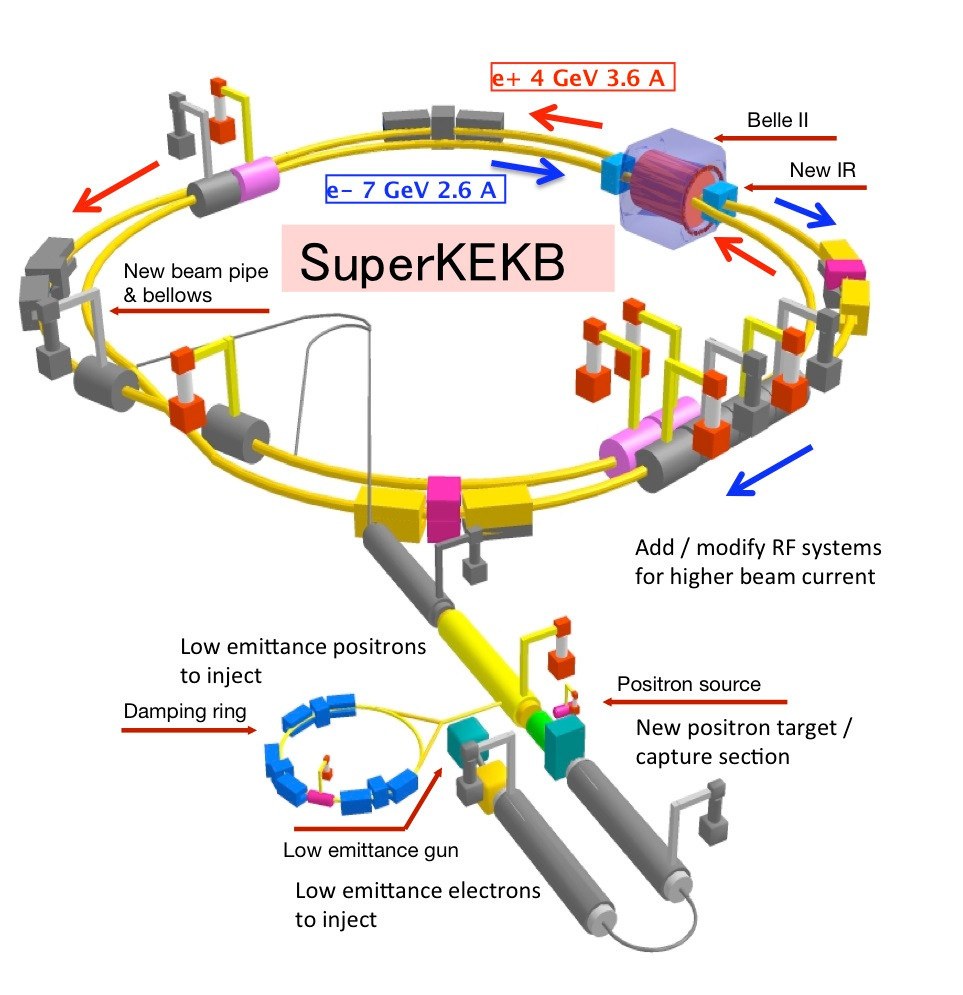
\includegraphics[height=0.4\textheight]{figures/experimental_setup/superkekb.jpg}
 \caption[Sketch showing the SuperKEKB electron--positron collider.]{Sketch showing the SuperKEKB electron--positron collider with the Belle~II detector. Taken from~\cite{DesyWebseite}.}
 \label{fig-superkekb}
\end{figure}


The Belle~II detector is used for measuring the products of the electron--positron collisions produced by the two-ring asymmetric-energy SuperKEKB collider. A sketch of the collider can be found in figure~\ref{fig-superkekb}. Like its predecessor, KEKB, its center of mass energy is tuned to be near the $\PgUc$ resonance. This beam energy is chosen because a $\PgUc$ particle decays with a branching fraction of 96 \% into a pair of entangled B-mesons. As described in the introduction, the daughter particles of these B mesons open a window to a very wide range of physical studies such as CP violation, analysis of rare decays or meson spectroscopy. The energy of the colliding electrons and positrons is asymmetric -- $\unit[4]{GeV}$ for the positrons and $\unit[7]{GeV}$ for the electrons -- which leads to a boosted center-of-mass-system along the beam axis. This fact is exploited when measuring the decay length of the two formed B-Mesons -- one of the main ingredients for quantifying the CP violation in the B Meson system and for identification of short-lived particles. 

The usage of electrons and their antiparticles for collisions leads to very clean events compared to other collision partners like protons or even gold atoms. Clean in this context means that a reduced number of created decay products (only 11 charged tracks on average) and no pile up (the number of collisions per bunch are well below one) are expected. These circumstances can be used for high-precision measurements on the formed particles.

As every general-purpose high energy physics particle detector the Belle~II detector is composed of several individual measuring devices -- each one with a different task -- arranged in different layers from the interaction point going outwards. The detector consists of basically six measuring components:
\begin{zlist}
  \item two layers of silicon pixel detectors for measuring the charged particles near the interaction point (PXD),
  \item four layers of doubled-sided silicon strip layers (SVD) with nearly the same purpose as the PXD,
  \item the central drift chamber (CDC) for measuring the momentum and the charge of charged particles,
  \item a time-of-propagation counter (TOP) together with the endcap particle identification detector (aerogel ring imaging Cherenkov detector, ARICH) for identification of the produced particles using Cherenkov radiation,
  \item an electromagnetic calorimeter (ECL) built of scintillating CsI(Tl) crystals for measuring the energy of mostly photons and electrons,
  \item and the K-long and muon detector (KLM) identifying these particle types in the outer region of the detector to improve the overall particle identification.
\end{zlist}

\section{The Tracking Detectors}

For collecting information on the physical process in the collision, details on the created decay products are needed. These include
\begin{zlist}
 \item Identification of the type of the created particles (e.g. by their mass),
 \item Measurement of the kinematic properties (e.g. momentum and energy) of the charged particles,
 \item Determination of their production vertex.
\end{zlist}

The tracking detectors described in this thesis are mainly built for recording the momenta of the particles as well as the position of their trajectories. The position information can then be used for combining two or more particles which originate from the same particle for measuring their vertex position. This vertex position is needed, for example, for measuring the CP violation in the B-meson system. % but also to distinguish between different particle types as the distance between the primary and the secondary vertex is proportional to the life time of the decaying particles. %Further more special applications are identification of the particle type by their energy loss.

By letting the charged particles fly through a sensor region, the parameters of the trajectories are measured . These sensors create space-resolved measurements and the full path of the particles through the detector -- a so called track -- can be obtained by combining the different location information -- the so called hits -- after the readout via software algorithms. By applying a magnetic field parallel to the beam axis\footnote{The coordinate system in Belle~II is chosen as the typical one in high energy particle physics~\cite{coordinate}: The $z$-axis is parallel to the beam axis with positive values in the boost direction whereas the $x$- and $y$-axis span a plane perpendicular to the beam line. The origin is the interaction point. Most of the time, one uses $r = \sqrt{x^2 + y^2}$ and $\phi = \arctan(y/x)$ rather than $x$ and $y$ directly because of the cylindrical symmetry of the detector.} -- the Belle~II nominal field strength is $B = \unit[1.5]{T}$ -- the charged particles curl. Measuring the curvature of the curled tracks gives an estimation of the momentum in the plane perpendicular to the beam axis -- the $r$--$\phi$-plane. The remaining $z$-direction parallel to the beam axis can be computed with the angle of the track to the beam axis. This procedure is described in more detail in chapter~\ref{chapter-theory}.

Many different ways exist to detect the passage of a charged particle through a sensor. Each of them exploits the charge of the particles and their interaction with materials which makes these techniques unusable for neutral particles. The vertex positions and momenta of uncharged particles can not be measured with the methods presented here. In Belle~II the momenta of neutral particles are resolved by assuming momentum conservation or by measuring the energy of photons in the calorimeter.\footnote{Photons are an example for neutral particles that deposit energy in the electromagnetic calorimeter as well. Their full trajectory can not be measured by the tracking detectors.} In the following, three tracking devices for charged particles are described in more detail. The main part (chapter~\ref{chapter-theory} and~\ref{chapter-workflow}) of this thesis covers the tracking in the CDC detector. Only chapter~\ref{chapter-vxd} on the VXD momentum estimation for slow pions uses the tracking in the PXD and SVD. As the implementation details of the VXD track finding are not relevant for the analysis presented there, the reconstruction software for the vertex detectors is not described here. Detailed information can be found elsewhere~\cite{jakob}.

All tracking detectors are built to cover the whole $\phi$ range of the detector and the acceptance region of $17-150 ^\circ$ in $\theta$ from forward to backward direction. The acceptance region can not cover the full $\theta$ range as the space for the beam pipe and the final focusing quadrupole magnets can not be covered with detecting devices. Once again the asymmetry in the $\theta$-acceptance reflects the boost in the positive $z$ direction induced by the asymmetric particle energies. The best momentum and position resolution can be obtained by combining the measured tracks in all three tracking detectors which is done after reconstructing the particles in the CDC and the combination of the two VXD detectors separately for improving the efficiency. The efficiency is increased when running the standalone track finders instead of building one track finder for all sub detectors, as the specialized algorithms can respond to specific properties of the detectors like the high occupancy in the VXD or the non-zero probability for missing hits in the CDC more easily. 

\subsection{Central Drift Chamber (CDC)}

With its radius of about $\unit[1.3]{m}$ the CDC is the largest and outer-most tracking detector in Belle~II. The CDC is a multi-wire proportional chamber detector with 14336 sense wires arranged in 56 layers grouped in 9 superlayers. These sense wires, together with a larger number of field wires, are strained mostly parallel to the beam axis in a cylindrical tank flooded with gas which spreads over the whole detector in the acceptance range. The gas is a mixture of 50 \% helium and 50 \% ethane. For more information on gas chamber detectors see for example reference~\cite{grupen}.

Each charged particle produced in the collision of the electron and positron with a transverse momentum high enough to exit the inner VXD detectors, interacts with the gas and can ionize the helium atoms. The energy deposition of a charged particle (except for electrons) is given by the Bethe formula~\cite{bethe}
\begin{align}
 - \left\langle \dd{E}{x} \right\rangle = K z^2 \frac{Z}{A \beta^2} \left( \frac 1 2 \frac{2 m_e c^2 \beta^2 \gamma^2 E_\text{max}}{I^2} - \beta^2 - \frac{\delta(\beta \gamma)}{2}  \right) \ , \label{form-bethe}
\end{align}
which describes the average energy loss per travel length. $K$, $z$, $Z$, $A$ and $I$ are material dependent constants, $\beta$ and $\gamma$ are the well-known kinematic variables. $E_\text{max}$ describes the maximal energy transfer to the absorber and $\delta$ the Fermi correction due to density effects. The described energy is transfered to the shell electrons of the helium gas atoms. As the ionization energy of helium is very low (about $\unit[20]{eV}$) the helium atoms release their electrons very easily. These free electrons get accelerated in an artificial electric field. This electric field is induced by applying a high voltage between sense and field wires. An instructive simulation of the typical electric field distribution between 7 sense wires and 34 field wires can be found in figure~\ref{fig-sense-wires}. Caused by the electric field configuration, the field strength near the sense wires increases strongly. The free electrons are accelerated in this increasing electrical field until they have enough kinematic energy to ionize helium atoms by themselves. This amplified cloud of free charge can be detected by the electronics attached to the sense wires and produce a sharp peak there. The immobile helium atomic cores receive their missing electron again later by the field wires. The additional fraction of ethane in the gas cells ensures that the cascading ionization is localized in the sense wire region.

Because the free electrons have to drift through the gas, the measured signal has a delay of up to $\unit[500]{ns}$ for the largest drift cells to the initial charged particle passage. By analyzing the time and location information of each measured signal, the path of the charged particle through the CDC can be reconstructed. A typical event display of the simulated passage of ten charged pions with $\unit[1]{GeV}$ can be seen in figure~\ref{fig-event-display}. As the electric charge configuration in each drift cell is almost rotationally symmetric, each wire produces a so called drift circle rather than a single hit point, which can also be seen in the figure. The two-dimensional position of the particles in each drift cell can not be measured, as only a one-dimensional time difference is available.

If all CDC wires were strained perfectly in parallel to the beam axis in $z$-direction, there would be no possibility to measure the $z$-information, e.g. the angle between the charged particles and the beam axis. That is the reason why some of the wires are installed with a small tilting angle with respect to the beam axis\footnote{Strictly speaking, the end-caps with the mounted wires get twisted not tilted, but as the twisting angle is small, there is not much difference in the two descriptions. Therefore the tilting is chosen which is much easier to imagine.}. These wires are called stereo wires in contrast to the axial wires without tilting angle. A measured hit on the stereo wires alone does give information neither on the position along the beam axis nor in the layer perpendicular to it as there is no possibility to measure the position along the wire where the particle passed by. Only the information collected among axial and stereo hits together lead to a correct estimation of the momentum in all directions as the axial wires define the position on the $r$--$\phi$-plane which in turn can be used to calculate the $z$-information with the stereo wires. A sketch of axial and stereo wires sharing the same distance from the beam axis -- also called a layer of wires -- is shown in figure~\ref{fig-axial-stereo}. 

The particle reconstruction has to take care of this special wire arrangement. First the axial hits are used for reconstructing the $r$--$\phi$-positions of the hits and the transverse momentum of the track. This information can be used with the stereo hits to obtain the $z$-momentum and by combining the tracks with the VXD tracks also the very important value of the $z$-distance between interaction point and track. The track finding algorithms also have to take into account the drift circle information for refining the track position. Each particle producing a hit must touch the drift circle tangentially. This can be used for finding all hits produced by the same particle (see chapter~\ref{chapter-theory}).

\begin{SCfigure}
  \caption[Simulation of the electric field in the central drift chamber.]{Simulation of the electron field in a fraction of the wires in the central drift chamber. The violet circles depict the field wires whereas the small red points are the sense wires. The yellow paths are examples for the drift paths of ionized electrons. This simulation includes the distortion by the magnetic field of the Belle II detector. Taken from~\cite{cdc_design}.}
  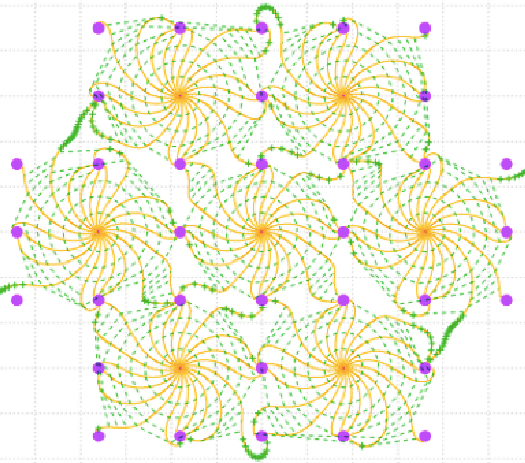
\includegraphics[width=0.5\linewidth]{figures/experimental_setup/electronsInCDC.pdf}
  \label{fig-sense-wires}
\end{SCfigure}

\begin{figure}
  \centering
  \begin{tikzpicture}
    \node[anchor=south west, inner sep=0] at (0,0) {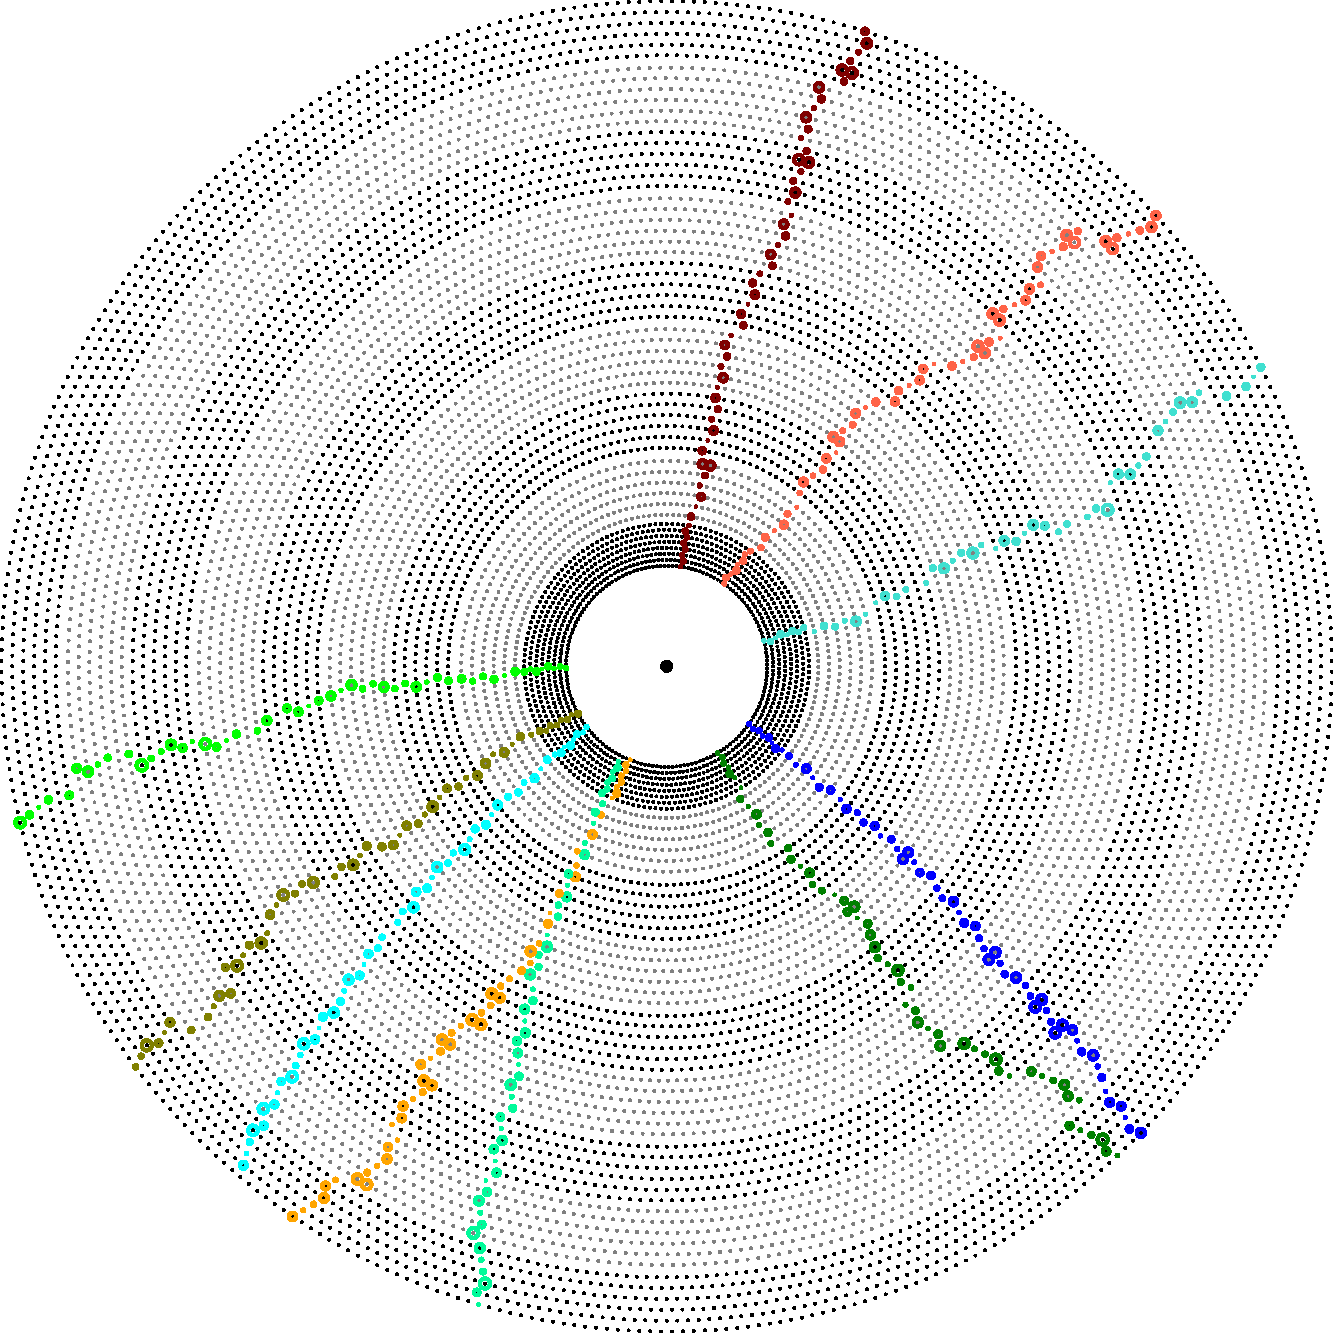
\includegraphics[width=0.8\linewidth]{figures/experimental_setup/eventDisplayPionGun.pdf}};
    \draw[black, rounded corners, fill=white] (-0.9, 6.9) rectangle (5.1, 12.9);
    \node[anchor=south west, inner sep=0] at (-0.8, 7) {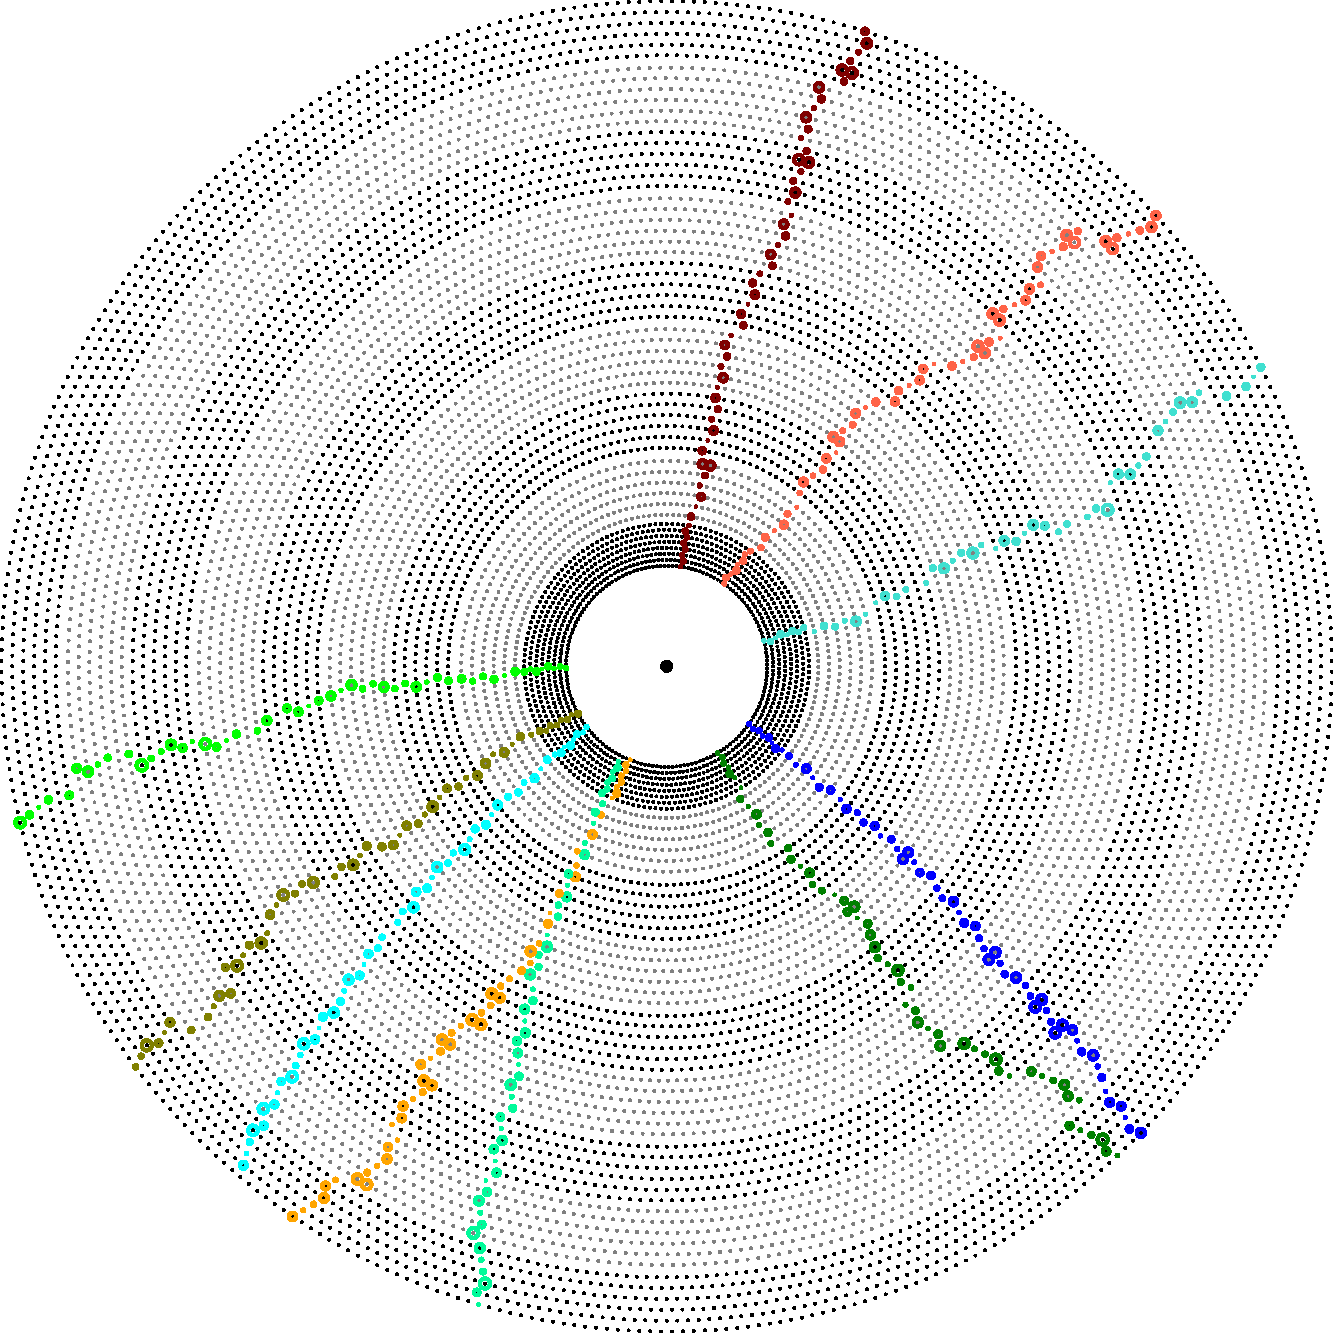
\includegraphics[trim={4cm 4cm 12.8cm 12.8cm}, clip, scale=1]{figures/experimental_setup/eventDisplayPionGun.pdf}};
  \end{tikzpicture}
  \caption[Simulated event of the passage of 10 $\Ppi^\pm$ through the CDC.]{Simulated event of the passage of 10 $\Ppi^\pm$ with approximately $\unit[1]{GeV}$ through the CDC shown in a plane perpendicular to the beam axis. The interaction point is drawn as a black circle in the center. Each particle is colored differently to distinguish between them. Only the CDC detector is shown for better visibility. The wires are shown as gray (stereo) or black (axial) points. The hit wires are depicted with their drift circles. The apparent disruption in the circular paths of the particle arises due to the tilting angle of the stereo wires with respect to the axial wires.}
  \label{fig-event-display}
\end{figure}

\begin{figure}
  \centering
  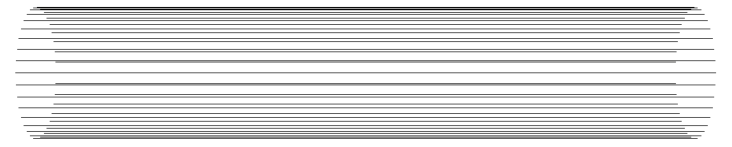
\includegraphics{figures/experimental_setup/axialLayers.pdf}
  
  \vspace*{1.5cm}
  
  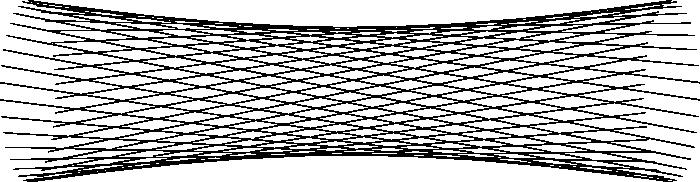
\includegraphics{figures/experimental_setup/stereoLayers.pdf}
  \caption[Sketch of the axial (top) and stereo wires in the CDC.]{Sketch of the axial (top) and stereo wires in the CDC. The skewing against the beamline of the stereo (bottom) wires is exaggerated. Taken from~\cite{oliver}.}
  \label{fig-axial-stereo}
\end{figure}

\subsection{Vertex Detectors (VXD)}
The term VXD refers to the two VerteX Detectors: the PiXel Detector (PXD) and the Silicon Vertex Detector (SVD). These two detectors are the innermost tracking detectors and are therefore used for measuring low momentum particles that do not reach into the CDC. The vertex and momentum resolution of all produced decay products is increased by combining the measured particle trajectories from the CDC with a good momentum resolution and the VXD with a good vertex resolution later.

The PXD consists of two layers of over eight million depleted field effect transistor (DEPFET) pixels made of silicon. Because the ASICs-built readout electronics is located outside of the acceptance region of the detector, the non-sensing material budget close to the interaction region is reduced. This, however, increases the readout time to over $\unit[20]{\mu s}$ also. The DEPFET technology makes it possible to build very thin (approximately $\unit[75]{\mu m}$) sensors which reduces multiple scattering. The thin sensors consume very little power making $\mathrm{CO}_2$ cooling sufficient. Strip sensor with a similar spatial resolution would lead to a much higher material budget.

The pixels are grouped into two layers of sensors at radii of $\unit[14]{mm}$ and $\unit[22]{mm}$. The two layers consist of 8 and 12 sensor panels with a width of $\unit[15]{mm}$ and a sensitive length of $\unit[90]{mm}$ and $\unit[123]{mm}$ leading to the typical acceptance region of 17 (forward) to 150 (backward) degrees which is used throughout the whole detector setup. The readout-electronics are mounted at the end of each layer and are connected to the data acquisition system outside the detector by optical fibers.

Each pixel consists of a fully depleted p-channel MOSFET (or JFET) with an artificial potential minimum (also called internal gate) just under the transistor channel induced by additional phosporus depletion. Incident particles generate electron--hole pairs in the n-bulk. The electrons drift towards this internal gate. When switching the p-channel MOSFET on, these accumulated electrons change the electronic behavior of the transistor which can be measured by the external electronics. The measurement is non-destructive -- therefore the signal electrons have to be ``cleared'' from the internal gate by a high-voltage punch-through. A cross-section of one pixel is shown in figure~\ref{fig-pxd-schema}.

\begin{figure}
  \centering
  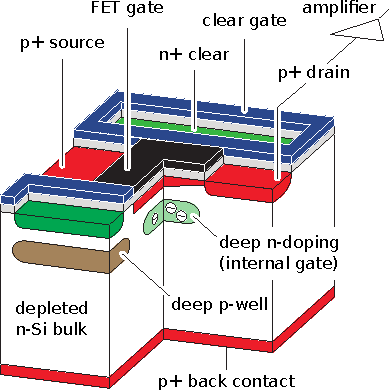
\includegraphics[width=0.6\linewidth]{figures/experimental_setup/pxd.pdf}
  \caption[Cross-section of a PXD sensor]{Schematic cross-section of on PXD sensor pixel of the Belle~II detector with the different parts as described in the text. Taken from~\cite{tdr}.}
  \label{fig-pxd-schema}
\end{figure}


The SVD is built of four layers of double-sided silicon strip sensors. The main task of the SVD is to connect the measurements from the PXD, the innermost detector, with the CDC measurements. However it is also possible to perform a SVD-standalone tracking in Belle~II which can improve the efficiency for very-low momentum particles that do not reach the CDC\footnote{The minimal transverse momentum to reach the CDC is defined by the magnetic field strength and the inner radius of the CDC. Because of material effects it differs for different particle types. The typical minimal momentum is in the region of some tens of MeV.}. The four layers have radii from 38 to 140 mm and therefore fill the gap between the PXD and the CDC detector. The 187 distinct sensors cover the whole acceptance region. As can be seen in figure~\ref{fig-belle2} and~\ref{fig-cluster-position} in chapter~\ref{chapter-vxd}, the sensors in the forward direction of the detector are constructed with a small slope of about $15^\circ$ because in this direction the bigger part of the decay products is expected. 

The sensors in the SVD consist of double-sided 12-cm-long strips with pitch sizes of approximately $\unit[50]{\mu m}$ on the p-side and $\unit[200]{\mu m}$ on the n-side. As multiple scattering is the main issue in this measurement region, the thickness is an important factor, with $\unit[320]{\mu m}$ for the barrel and $\unit[300]{\mu m}$ for the slanted forward sensors. The measuring process is similar to the one in the PXD sensors. Particles passing through the sensor strips produce electron--hole pairs in the depleted region which get measured by the external electronics. 

As can be seen, the sensors with the best spatial resolution are located closest to the interaction point. All three presented detectors are a trade-off between good positional measurement, low read-out time, low material budget and in the end also low price. The innermost detectors have to cope with the highest radiation and also the highest amount of expected background hits whereas the CDC as the largest detector is responsible for improving the momentum resolution with as many hits as possible and a larger lever arm.

\subsection{Beam-Induced Background in the Tracking Detectors}

The expected luminosity of SuperKEKB will be 40 times higher than at KEKB~\cite{tdr}. Increasing the beam current and reducing the beam sizes at the interaction point however also causes higher beam-induced background which can impede the measurements in the tracking detectors and the track finding. In the following, the five main sources of expected beam-induced background are described. The expected background is higher for the VXD, as the distance to the interaction point is smaller. More information can be found in reference~\cite{jakob}. The background mitigation techniques in the software for the CDC track finding are described in chapter~\ref{chapter-workflow}.

\begin{description}
 \item[Synchrotron Radiation (SR)] The electron and positron bunches in the high energy storage ring at SuperKEKB emit synchrotron radiation because of their bent trajectories in the magnets. The energy of the created photons can be high enough for ionization processes. The synchrotron radiation in the Belle~II detector is even worse than in the rest of the storage ring, because of the strong focusing magnets in front of the interaction point. A special construction of the IP chamber design can help to reduce this background source.
 \item[Beam-Gas Scattering] Interactions of the beam particles with residual gas in the beam pipe (bremsstrahlung and Coulomb scattering) leads to momentum changes of the electrons and positrons. As the deflection in the bending magnets is momentum dependent, these particles can then hit the wall of the vacuum chambers and magnets producing showers of secondary particles which can enter the detectors.
 \item[Touchek Scattering] Intra-bunch scattering can lead to the same momentum changes as the beam-gas scattering described before with the same anticipated consequences.
 \item[Radiative Bhabba Scattering] In most of the cases the colliding electron and positron do not create a Y(4S) -resonance but rather interact via Bhabba scattering. The produced photons and the electron--positron-pair can lead to secondary particle showers.
 \item[Electron--Positron Pair Production] Low momentum electron--positron-pair background produced via $\Pep \Pem \to \Pep \Pem \Pep \Pem$ can lead to up to 14000 $\Pem\Pep$-pairs in each event in the first PXD layer leading to an increased occupancy in this layer.
\end{description}
